% This must be in the first 5 lines to tell arXiv to use pdfLaTeX, which is strongly recommended.
\pdfoutput=1
% In particular, the hyperref package requires pdfLaTeX in order to break URLs across lines.

\documentclass[11pt]{article}

% Change "review" to "final" to generate the final (sometimes called camera-ready) version.
% Change to "preprint" to generate a non-anonymous version with page numbers.
\usepackage[preprint]{mtsummit25}

% Standard package includes
\usepackage{times}
\usepackage{latexsym}

% For proper rendering and hyphenation of words containing Latin characters (including in bib files)
\usepackage[T1]{fontenc}
% For Vietnamese characters
% \usepackage[T5]{fontenc}
% See https://www.latex-project.org/help/documentation/encguide.pdf for other character sets

% This assumes your files are encoded as UTF8
\usepackage[utf8]{inputenc}

% This is not strictly necessary, and may be commented out,
% but it will improve the layout of the manuscript,
% and will typically save some space.
\usepackage{microtype}

% This is also not strictly necessary, and may be commented out.
% However, it will improve the aesthetics of text in
% the typewriter font.
\usepackage{inconsolata}

%Including images in your LaTeX document requires adding
%additional package(s)
\usepackage{graphicx}

% If the title and author information does not fit in the area allocated, uncomment the following
%
%\setlength\titlebox{<dim>}
%
% and set <dim> to something 5cm or larger.

% custom packages
\usepackage[british]{babel}
\usepackage[babel]{csquotes}
\usepackage{booktabs}
\usepackage{tabularx}
\usepackage{xurl}



% References inside the document
\newcommand{\see}[1]{(see #1)}
\newcommand{\Chapter}[1]{Chapter~\ref{chap:#1}}
\newcommand{\Appendix}[1]{Appendix~\ref{chap:Appendix#1}}
\newcommand{\Section}[1]{Section~\ref{sec:#1}}
\newcommand{\Table}[1]{Table~\ref{tab:#1}}
\newcommand{\Figure}[1]{Figure~\ref{fig:#1}}
\newcommand{\Eq}[1]{Equation~\eqref{eq:#1}}
\newcommand{\Eqp}[1]{(Equation~\ref{eq:#1})}


\title{A comparison of translation performance between DeepL and Supertext}


\author{
 \parbox{0.75\linewidth}{\centering
     \textbf{Alex Flückiger},
     \textbf{Chantal Amrhein},
     \textbf{Tim Graf},
     \textbf{Frédéric Odermatt},
     \textbf{Martin Pömsl},
     \textbf{Philippe Schläpfer},
     \textbf{Florian Schottmann},\\
     \textbf{Samuel Läubli}}
     \vspace{0.6em}
\\
 Supertext
 \vspace{0.6em}
\\
 \texttt{\{firstname.lastname\}@supertext.com}
}


\begin{document}
\maketitle 
\begin{abstract}
As strong machine translation (MT) systems are increasingly based on large language models (LLMs), reliable quality benchmarking requires methods that capture their ability to leverage extended context. This study compares two commercial MT systems -- DeepL and Supertext -- by assessing their performance on unsegmented texts. We evaluate translation quality across four language directions with professional translators assessing segments with full document-level context. While segment-level assessments indicate no strong preference between the systems in most cases, document-level analysis reveals a preference for Supertext in three out of four language directions, suggesting superior consistency across longer texts. We advocate for more context-sensitive evaluation methodologies to ensure that MT quality assessments reflect real-world usability.\footnote{We release all evaluation data and scripts for further analysis and reproduction at \url{https://github.com/supertext/evaluation_deepl_supertext}}
\end{abstract}

\section{Introduction}
\label{sec:Introduction}
After the transition from statistical to neural modelling roughly a decade ago 
\citep{Kalchbrenner2013,Sutskever2014,Bahdanau2015}, the field of MT is undergoing another paradigm shift towards leveraging LLMs \citep{xu2024paradigmshiftmachinetranslation,wu2024adaptinglargelanguagemodels,kocmi-etal-2024-findings}. LLM-based translation offers the potential for significantly improved translation quality, especially with respect to consistent translation of documents. Unlike neural machine translation (NMT) systems, which typically process documents as isolated sentences or paragraphs \citep{Post2023EscapingTS}, many LLMs operate with context windows that can span thousands of words, allowing them to maintain consistency throughout a document -- for instance, by ensuring that a word’s translation in the final sentence matches its previous forms \citep{wu2024adaptinglargelanguagemodels}.

In the most recent shared task at the Conference on Machine Translation (WMT24) that focuses on evaluating the state of the art in general-domain translation quality, the majority of the 28 system submissions were already based on LLMs \citep{kocmi-etal-2024-findings}. 
Although without statistical significance and for the language direction English to German only, one system even outranked the human reference translations as evaluated by professional human annotators.

Despite this impressive achievement, findings of human-machine parity should be approached with caution. Similar claims already emerged with pre-LLM technology \citep{hassan2018achieving}, yet have subsequently been refuted due to limitations in the evaluation design focusing on single segments in isolation \citep{laubli-etal-2018-machine,toral-etal-2018-attaining, freitag-etal-2021-experts}. The WMT24 shared task also highlights that evaluations based on automatic metrics (rather than human evaluation) can lead to wrong conclusions when comparing strong MT systems \citep{kocmi-etal-2024-findings}.

However, these insights are often overlooked in evaluations of commercial MT systems. For example, Intento's The State of Machine Translation 2024 report,\footnote{\label{Intento}\url{https://inten.to/machine-translation-report-2024}} which assesses 52 providers across 11 language pairs, serves as a valuable resource for potential users in real-world settings, but its benchmarking methodology relies on automatic scoring of sentence-level data, and the authors acknowledge that \enquote{you may need a human linguist} to ensure greater reliability.

In this paper, we evaluate two commercial translation systems (\Section{Systems}) under conditions that allow for leveraging the full-text capabilities of LLMs. Source texts are translated without prior segmentation (\Section{Data}), and the resulting translations are rated by professional translators considering the full document context (\Section{EvaluationSetup}). We find that while both systems translate a similar number of segments better than the other, the difference is more pronounced on the document level (\Section{Results}), which we attribute to differences in how much context the systems consider during translation (\Section{Discussion}). Our findings suggest that the adoption of LLMs creates opportunities for smaller players to challenge dominant industry leaders (\Section{Conclusion}).


\section{Systems}
\label{sec:Systems}

We compare the free online offering of two commercial MT providers:

\paragraph{DeepL}
DeepL\footnote{\url{https://www.deepl.com}} is a widely used MT provider boasting \enquote{unrivalled translations that set the standard}.\footnote{\label{DeepLQuality}\url{https://www.deepl.com/en/quality}} In the latest Intento report, it scores best among nine \enquote{real-time engines} and, together with GPT-4, is found to \enquote{consistently outperform other models}.\footref{Intento} Due to its closed source, the technology behind DeepL's translation system is not publicly known.

\paragraph{Supertext} 
Supertext\footnote{\url{https://www.supertext.com}} builds on an open, general-purpose LLM that has been specialised for the task of translation with proprietary methods and data. While the system can be adapted to specific domains, we use the freely available generic version.

\vspace{1em}

\noindent For the purpose of the evaluation described in this paper, we use both systems with default settings. For example, we do not specify politeness (formal/informal) although supported by both systems in some language combinations.

While both DeepL and Supertext provide target language variants for English (British and American), Supertext also provides target language variants for German (Austria, Germany, Switzerland), French (France, Switzerland), and Italian (Italy, Switzerland). We use a specific target language variant whenever available (\Section{TargetTexts}).


\section{Data}
\label{sec:Data}

\subsection{Source Texts}
\label{sec:SourceTexts}

We collect 20 texts each in two source languages: English (en) and German (de). All texts stem from news websites: New York Times\footnote{\url{https://www.nytimes.com}} for English and Neue Zürcher Zeitung\footnote{\url{https://www.nzz.ch}} for German, respectively. We select 10 FAQ pages and 10 recent news articles in the economy section from each website. To balance the distribution of text lengths, we crop the end of some texts omitting their final paragraphs. Notably, these texts are only available in a single language; they are unlikely to be contained in the training data of either system we evaluate.

\subsection{Target Texts}
\label{sec:TargetTexts}

We create translations in four language directions (\Table{data_stats}) directly in the respective online translation interface of each system as a regular user would.\footnote{All translations were produced on 27 January 2025.} We do not modify the texts before translation and paste them in their original formatting, including newlines.

After translation, we manually split and align the source texts and translations into sentences. If one of the systems merges two or more sentences into a single sentence, we ensure that the same content is merged for the other system, such that the raters are presented with parallel segments. Table \ref{tab:data_stats} shows the number of segments per language pair.

\begin{table}[t]
    \centering
    \begin{tabular}{lrr}
        \toprule
        Language Direction & Texts & Segments\\
        \midrule
        de $\rightarrow$ en-GB & 20 & 281\\
        de $\rightarrow$ fr-CH & 20 & 276\\
        de $\rightarrow$ it-CH & 20 & 265\\
        en $\rightarrow$ de-CH & 20 & 211\\
        \bottomrule
    \end{tabular}
    \caption{Evaluation data by language direction.}
    \label{tab:data_stats}
\end{table}

\section{Evaluation Setup}
\label{sec:EvaluationSetup}

We conduct a blind A/B test in which professional translators rate DeepL and Supertext outputs with full document-level context.

\subsection{Raters}
\label{sec:Raters}

We enrol 8 professional translators with experience in evaluating machine translation output, 1 to 3 per language direction. All raters have between 2 and 19 years of professional experience (average=8.6 years) in the language combination they are assigned to and are native in the respective target language.


\subsection{Materials}
\label{sec:Materials}

We arrange all segments of a source document with their corresponding translations by both systems in a spreadsheet. The segments are presented in original document order, including formatting such as newlines, such that raters see the full source text and both translations side-by-side. We randomly assign the system outputs to columns labelled Translation A and Translation B for each text such that raters do not have any information about which translation stems from which system (a blind A/B test setting). Assignments are kept consistent within a text such that the document context remains natural.

\subsection{Procedure}
\label{sec:Procedure}

Documents are assigned to single raters. For each segment in each document, the assigned rater is asked to choose whether Translation A is better, Translation B is better, or whether both translations are of equal quality.

Our instructions explicitly state that \enquote{equal} can mean that two translations are equally good or equally bad. Moreover, the raters were asked to focus on the content rather than punctuation to avoid that the results get biased because of specifics of a language variant.

\section{Evaluation Results}
\label{sec:Results}

Segment-level and text-level preference ratings are shown in Figures~\ref{fig:by-segment} and~\ref{fig:by-text}, respectively.

\begin{figure}[t]
    \centering
    \includegraphics[height=4.48cm]{preferences_overall_rel_n.png}
    \caption{Segment-level ratings.}
    \vspace{2.3em}
    \label{fig:by-segment}
\end{figure}

\subsection{Segment-level}
\label{sec:ResultsSegmentLevel}
Across all language pairs, 9.5\% of the segments generated by DeepL and Supertext are identical. The overlap is highest in de $\rightarrow$ en-GB, particularly in the FAQ texts where 26.1\% of the segments were translated identically.

Participants rate most segments as equal in terms of translation quality in three out of four language directions. While the number of segments where one system is preferred over the other is similar for DeepL and Supertext in these language directions, raters show a preference for DeepL in en $\rightarrow$ de-CH (88~DeepL, 66~equal, 57~Supertext).

\subsection{Document-level}
\label{sec:ResultsDocumentLevel}
We derive document-level preferences by aggregating the segment-level ratings of each evaluated document. For example, a text is counted as \enquote{DeepL better} if the rater preferred DeepL's translations for more segments than Supertext's translations in that document.

In contrast to the pooled segment-level ratings (\Section{ResultsSegmentLevel}), raters show a preference for documents translated by Supertext in three out of four language directions, most notably in de $\rightarrow$ it-CH (7~DeepL, 3~equal, 10~Supertext). In en $\rightarrow$ de-CH, however, raters show a clear preference for documents translated by DeepL (13~DeepL, 2~equal, 5~Supertext).

\begin{figure}[t]
    \centering
    \includegraphics[height=4.48cm]{preferences_by_text_rel_n.png}
    \caption{Aggregated segment-level ratings per text. Texts with the same number of preferred segments for both systems are excluded.}
    \label{fig:by-text}
\end{figure}

\begin{table*}[t]
    \tiny
    % !TEX root = main.tex

\begin{figure}[t]
\vspace{-1.5cm}
\begin{minipage}{0.34\textwidth}
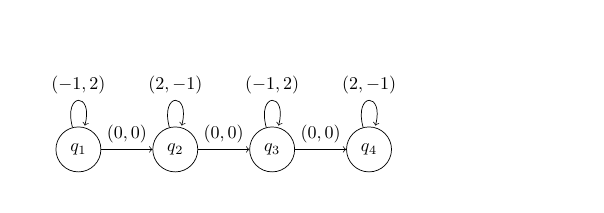
\begin{tikzpicture}[scale=0.25]
\usetikzlibrary{automata, positioning}
\scalebox{0.65}{
\node[state] (q1) {$q_1$};
\node[state, right=of q1] (q2) {$q_2$};
\node[state, right=of q2] (q3) {$q_3$};
\node[state, right=of q3] (q4) {$q_4$};

\path[->] (q1) edge [loop above] node[above] {$(-1,2)$} (q1) edge node[above] {$(0,0)$} (q2); 
\path[->] (q2) edge [loop above] node[above] {$(2,-1)$} (q2) edge node[above] {$(0,0)$} (q3);
\path[->] (q3) edge [loop above] node[above] {$(-1,2)$} (q3) edge node[above] {$(0,0)$} (q4);
\path[->] (q4) edge [loop above] node[above] {$(2,-1)$} (q4);
}
\end{tikzpicture}
\end{minipage}
\begin{minipage}{0.32\textwidth}
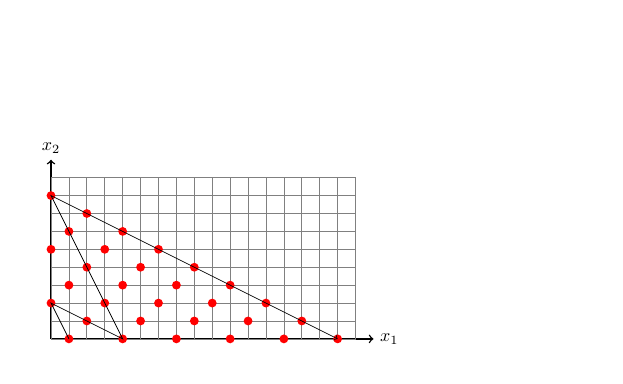
\begin{tikzpicture}[scale=0.35]
\scalebox{0.65}{
\draw[->, thick] (0, 0) -- (18, 0) node[right] {$x_1$};
\draw[->, thick] (0, 0) -- (0, 10) node[above] {$x_2$};

\draw[step=1, gray, thin] (0, 0) grid (17, 9);

\foreach \x in {1,4,7,10,13,16} \fill[red] (\x,0) circle (7pt);
\foreach \x in {2,5,8,11,14} \fill[red] (\x,1) circle (7pt);
\foreach \x in {0,3,6,9,12} \fill[red] (\x,2) circle (7pt);
\foreach \x in {1,4,7,10} \fill[red] (\x,3) circle (7pt);
\foreach \x in {2,5,8} \fill[red] (\x,4) circle (7pt);
\foreach \x in {0,3,6} \fill[red] (\x,5) circle (7pt);
\foreach \x in {1,4} \fill[red] (\x,6) circle (7pt);
\foreach \x in {2} \fill[red] (\x,7) circle (7pt);
\foreach \x in {0} \fill[red] (\x,8) circle (7pt);

\draw[->] (1,0) -- (0,2) -- (2,1) -- (4,0) -- (3,2) -- (2,4) -- (1,6) -- (0,8) -- (2,7) -- (4,6) -- (6,5) -- (8,4) -- (10,3) -- (12,2) -- (14,1) -- (16,0);
}
\end{tikzpicture}
\end{minipage}
\begin{minipage}{0.32\textwidth}
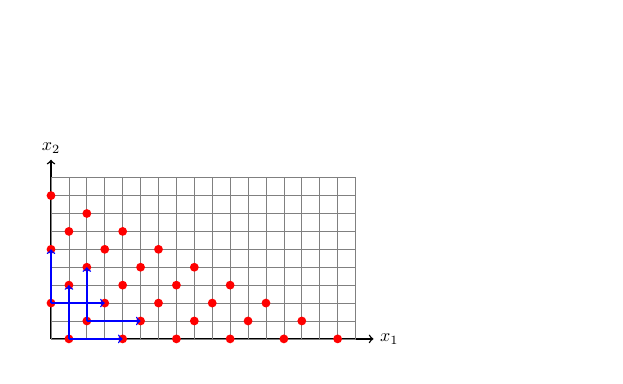
\begin{tikzpicture}[scale=0.35]
\scalebox{0.65}{
\draw[->, thick] (0, 0) -- (18, 0) node[right] {$x_1$};
\draw[->, thick] (0, 0) -- (0, 10) node[above] {$x_2$};

\draw[step=1, gray, thin] (0, 0) grid (17, 9);

\foreach \x in {1,4,7,10,13,16} \fill[red] (\x,0) circle (7pt);
\foreach \x in {2,5,8,11,14} \fill[red] (\x,1) circle (7pt);
\foreach \x in {0,3,6,9,12} \fill[red] (\x,2) circle (7pt);
\foreach \x in {1,4,7,10} \fill[red] (\x,3) circle (7pt);
\foreach \x in {2,5,8} \fill[red] (\x,4) circle (7pt);
\foreach \x in {0,3,6} \fill[red] (\x,5) circle (7pt);
\foreach \x in {1,4} \fill[red] (\x,6) circle (7pt);
\foreach \x in {2} \fill[red] (\x,7) circle (7pt);
\foreach \x in {0} \fill[red] (\x,8) circle (7pt);

\draw[->,blue,thick] (1,0) -- (4,0);
\draw[->,blue,thick] (1,0) -- (1,3);

\draw[->,blue,thick] (2,1) -- (5,1);
\draw[->,blue,thick] (2,1) -- (2,4);

\draw[->,blue,thick] (0,2) -- (3,2);
\draw[->,blue,thick] (0,2) -- (0,5);
}
\end{tikzpicture}
\end{minipage}
\caption{Left: 4-component \dvass $V_2$. 
Middle: the set $\reach_{q_4}(V_2, q_1(1,0))$ and a path $q_1(1,0) \tran q_4(16,0)$.
Right: bases 
%$A = \{(1,0),(2,1),(0,2)\}$ 
and periods 
%$P = \{(0,3),(3,0)\}$
 of an over-approximating semi-linear set $A+P^*$.}
\label{fig:zigzag}
\end{figure}

\begin{example}
For $k\geq 1$, let $V_k$ be a $(2k)$-component \dvass, where each component has just one state $q_i$
and one transition:
$(q_i, (-1,2), q_i)$ for odd $i$, and $(q_i, (2,-1), q_i)$ for even $i$.
Bridge transitions are $(q_i, (0,0), q_{i+1})$.
Figure~\ref{fig:zigzag} shows $V_2$ (left) and 
a path in $V_2$ from $s = q_1(1,0)$ to $t = q_4(16,0)$ together with 
the reachability set $\reach_{q_4}(V_2, s)$ (middle).
In general,
\begin{align} \label{eq:reachk}
X_k := \reach_{q_{2k}}(V_k, s) \ = \ \set{(x_1,x_2) \mid x_1+2x_2 \leq 4^k, \  x_1+2x_2 \equiv 1 \!\! \mod 3}.
\end{align}
Even if the size of the reachability set is 
exponential in $k$, for small $(x_1, x_2)$ it is periodic and the periods are small.
The set $X_k$ can be over-approximated by $A + P^*$ for $A = \set{(1,0),(2,1),(0,2)}$ and $P = \set{(0,3),(3,0)}$
(shown on the right of Figure~\ref{fig:zigzag}), namely for every $k\geq 1$ and $B\in\N$,
the set $X_k$ is \kanapka {$8$} {$B$}. 
For illustration, consider $Y := X_k \cap ((1,0) + P^*)$.
If $(1,0) + P^{\leq B} \subseteq X_k$ then $Y$ is a $B$-approximation
of $(1,0) + P^*$ with $\norm((1,0)), \norm(P) \leq 3 \leq 8$. 
Otherwise, there is some $(v_1, v_2) \in \big((1,0) + P^{\leq B}\big)\setminus X_k$, and
then $B$ is larger than $4^k$:
\[
%8B \geq 2(1 + 3B) \geq 2(v_1 + v_2) \geq v_1 + 2 v_2 > 
4^k < v_1 + 2 v_2 \leq 2(v_1 + v_2) \leq 2(1+3B) \leq 8B.
\]
Therefore by \eqref{eq:reachk}, each $(x_1,x_2) \in Y$ satisfies 
$\norm(x_1,x_2) = x_1 + x_2 \leq x_1 + 2x_2 \leq 4^k < 8B$, and thus
$Y$, seen as a union of singletons, is a union of 
linear sets with norm of base bounded by $8B$ and empty set of periods. 
In both cases, 
$Y$ is \kanapka {$8$} {$B$}. 
%The same intuition stays behind polynomial approximability of \dvass stated in Lemma~\ref{lem:2vass-sandwich}.
\end{example}
    \caption{Example of a rated de $\rightarrow$ en-GB document. Better-rated translations are highlighted in bold; segments without any bold translation were rated as equal. System names are not shown during evaluation (\Section{EvaluationSetup}).}
    \label{tab:example}
\end{table*}

\section{Discussion}
\label{sec:Discussion}
Our evaluation highlights that conclusions drawn from MT quality assessments may vary significantly depending on the unit of measurement. While raters in our study preferred a similar number of translated segments by DeepL and Supertext overall, the difference becomes more pronounced at the document level. This discrepancy suggests that segment-level assessments alone may not fully capture translation quality as perceived in real-world usage, where coherence and consistency across entire documents play a critical role.

Notably, while segment-level ratings indicate no strong preference between the two systems in most language directions, document-level aggregation reveals a more distinct pattern. Raters favour Supertext's translations at the document level in three out of four language directions, with the most pronounced difference observed in de $\rightarrow$ it-CH. This suggests that Supertext may provide better consistency or fluency across longer texts in these language directions. While we have yet to conduct a systematic qualitative comparison of system outputs, we find texts where the same word is translated differently by DeepL and consistently by Supertext across paragraphs. An example is shown in \Table{example}, where DeepL translates the German word \textit{Startseite} as either \textit{start page}, \textit{home page}, or \textit{Home page}.

In contrast, for en $\rightarrow$ de-CH, raters show a clear preference for DeepL at both the segment and document levels, indicating a potential strength of DeepL in handling this specific language combination. Our preliminary analysis is inconclusive at this point, but the Supertext outputs seem to contain a higher number of within-sentence errors such as wrong choices for individual words or omissions. Another hypothesis is that Supertext, which supports three different German target language variants, may introduce inconsistencies by mixing region-specific elements in translation outputs.

\section{Conclusion}
\label{sec:Conclusion}

Our study highlights the growing significance of document-level evaluations in MT quality benchmarking, especially as LLM-based systems leverage broader context windows to enhance translation consistency. While segment-level assessments suggest no clear preference between DeepL and Supertext in most of the language directions we examined, document-level aggregation reveals notable differences. Supertext is preferred in three out of four language pairs, where its translations exhibit greater consistency. In contrast, en $\rightarrow$ de-CH shows a clear preference for DeepL, possibly due to fewer within-sentence errors or differences in regional language handling.

As LLM-based MT systems continue to evolve, future studies should further investigate the impact of context length on commercial MT benchmarking campaigns. Insights into how different systems leverage context and resolve ambiguities will be essential for advancing evaluation methodologies and ensuring that translation systems meet real-world user expectations.


\section*{Limitations}
While A/B tests are commonly used for comparing two systems and a reliable basis for incrementally improving MT systems \citep{tang_2010, wu-etal-2024-evaluating-automatic}, 
they provide no insight into the severity of errors within a translation or across different systems compared to MQM ratings \citep{freitag-etal-2021-experts}. Moreover, some mistakes may be harder to spot than others during real-world usage when not being shown contrastively against an alternative translation. Similarly, the preference in an A/B test may not correlate with the effort needed for post-editing the translation. To address these questions, we plan to extend our evaluation efforts.

The evaluation was carried out by professional translators working for Supertext. Since the A/B assignments were randomized and anonymized, we do not assume any bias. Additionally, in the interest of transparency, we publicly share the complete dataset, including the source text, translations from each system, and the corresponding ratings.

Finally, the scope of this study is not exhaustive but is limited to a subset of language pairs, two domains, and a limited number of documents. Yet, we are providing details that go beyond what DeepL is sharing publicly.\footref{DeepLQuality}


\section*{Acknowledgments}
We thank all the professional translators involved for their support with this evaluation.

% Bibliography entries for the entire Anthology, followed by custom (mtsummit25) entries
\bibliography{anthology,mtsummit25}

\end{document}
